\chapter{Sistema Proposto}
\label{cap:Estrutura}

De modo a conceber a arquitectura do sistema de Monitorização de Rede orientado ao Processo (\textit{MRoP}), foi necessário conhecer, como os processos em nível utilizador interagem com o exterior através da rede.
Uma vez conhecida a arquitectura de rede do \textit{Linux}, tornou-se imprescindível compreender a forma, como se processa a comunicação e a monitorização de rede.

Assim, tendo em conta os factores anteriormente mencionados, neste capítulo irá ser apresentada a constituição do sistema de rede do \textit{Linux}, desde o momento do envio dos dados pelo processo até que estes chegam à interface de rede e vice-versa.
Considerando a abrangência desta visão, apenas serão focados os componentes essenciais da arquitectura, nomeadamente o descritor de processo, as familias de \textit{sockets}, a \textit{firewall}, o sistema de escalonamento de rede e a monitorização de rede.

Após esta visão geral do sistema de rede do \textit{Linux}, será apresentada a arquitectura proposta para o sistema de Monitorização de Rede orientado ao Processo (\textit{MRoP}).

\section{Arquitectura de rede em \textit{Linux}}
\label{sub:network}

Os processos são instâncias de programas, e estes num sistema multiprogramado partilham recursos.
Os processos necessitam de comunicar para obter dados, de modo a completar as suas execuções.
Estas comunicações podem ser efectuadas tanto internamente, como externamente ao sistema.
Em geral, as comunicações externas processam-se através de uma interface de rede, sendo necessário, para tal, criar canais de comunicação.
A(s) interface(s) de rede são recursos do sistema, as quais são partilhadas pelos diversos processos.
Esta partilha é efectuada pelo núcleo, pois apenas este é capaz de a efectuar correctamente.

\begin{figure}[htbp]
\centering
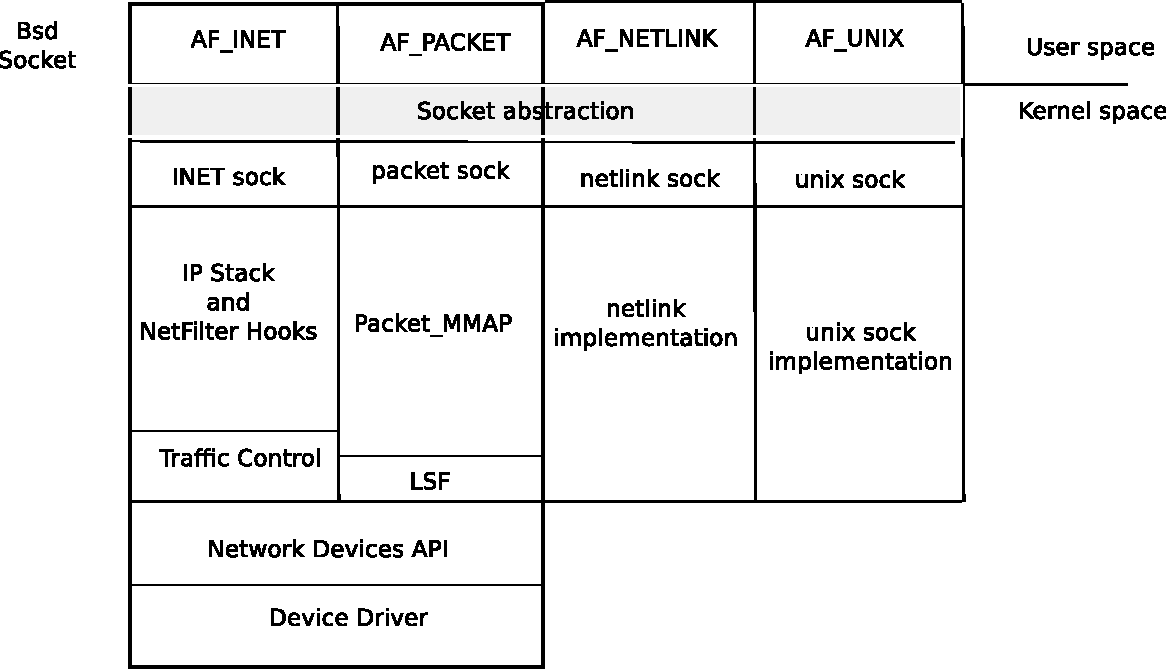
\includegraphics[scale=0.7]{network_arch.pdf} 
\caption{Arquitectura parcial de sockets do Linux}
\label{fig:network_arch}
\end{figure}

A chamada ao sistema \textit{socket}, é efectuada para a criação de um canal de comunicação e este varia em função dos parâmetros: família, tipo e protocolo.
Existe um agrupamento em família de endereços (\textit{Address Family}), que se destina à comunicação remota ou local.
Em termos gerais, as comunicações locais podem incidir na comunicação entre processos (\textit{AF\_UNIX}), ou entre estes e o núcleo (\textit{AF\_NETLINK}), enquanto as comunicações remotas podem ter lugar sobre a internet, dispondo igualmente de uma família própria para o efeito (\textit{AF\_INET}).
%As comunicações locais podem efectuar-se entre processos (\textit{AF\_UNIX}), ou entre estes e o núcleo (\textit{AF\_NETLINK}), enquanto as remotas podem ter lugar sobre a \textit{internet}, dispondo igualmente de uma família própria a \textit{AF\_INET}.
Estes canais possuem um conjunto de funções (\textit{API POSIX}) bem definidas, para utilização e controlo das operações, permitindo estruturar a comunicação de um modo eficiente.


%Para caracterizar o canal não é suficiente a especificação da família, é igualmente necessário especificar o tipo e o protocolo a utilizar, pois diferentes combinações de valores para estes parâmetros, traduzem-se em canais com diferentes funcionalidades.

Hoje em dia, os administradores de sistemas necessitam filtrar o fluxo de informação que circula nas suas redes.
Para tal, tem-se assistido ao desenvolvimento de sistemas de filtragem de comunicações, conhecidas por \textit{firewalls}.
Sendo o \textit{Linux} um sistema de operação frequentemente utilizado em ambientes de servidores, tornou-se essencial a aplicação deste tipo controlo.
Para tal a solulção encontrada resultou do desenvolvido de uma \textit{firewall} (a qual foi denominada por \textit{NetFilter}) capaz de filtrar o fluxo de dados que circula na rede, entre o sistema e a periferia.

Para além da existência da filtragem do fluxo de dados, o sistema de operação \textit{Linux} é constituido por um sistema de controlo do escalonamento do fluxo de tráfego, (\textit{Traffic Control}), que tal como o \textit{netfilter}, é definido no núcleo, permitindo ao administrador indicar quais os fluxos de dados prioritários ou que necessitam de determinada largura de banda, possibilitando-lhe efectuar uma reserva antecipada da mesma.
 
Adiante apresentar-se-ão diferentes constituintes da estrutura de rede do \textit{Linux}, iniciando-se pelo processo em nível utilizador terminando nos controladores de interfaces de rede.

Por último será apresentado o sistema de monitorização genérica de rede do \textit{Linux}.

\subsection{Estrutura de um processo}
% ou recursos de rede de um processo

Um processo é a instânciação de um programa, sendo igualmente uma unidade de escalonamento de execução (\textit{task}) no sistema operativo.
Este consome recursos (físicos e lógicos), partilhados com outros processos num sistema multiprogramado.
O núcleo de sistema gere uma estrutura para cada processo (\textit{struct\_task}), onde estão identificados todos os recursos a este atribuídos.
Esta estrutura contém apontadores para diversos recursos nomeadamente: zonas de memória requisitadas, canais abertos (ficheiros, \textit{sockets}, entre outros), contabilização de utilização de \textit{cpu}, apontadores para a sua árvore genealógica (pai, irmãos e filhos), etc.

A árvore genealógica anteriormente indicada contém o apontador para o processo pai (o processo que efectuou um \textit{fork}, para lhe dar origem), a lista de irmãos e dos descententes.
O processo pai, tal como cada um dos elementos presentes na lista, são também estruturas do tipo \textit{task\_struct}, possibilitando, desta forma, a navegação ao longo da árvore genealógica do processo.

Um dos recursos partilhados pelos diferentes processos é o acesso à rede, ou seja, o recurso que permite a comunicação com o exterior.
De modo a que as comunicações possam ter lugar, é necessário a alocação de canais de comunicação, cuja criação, utilização e destruição é efectuada pela \textit{API} definida no sistema de operação.
Quando um processo cria um canal, o núcleo devolve-lhe um identificador, que permitindo ao processo referenciar o canal dentro do núcleo e, deste modo, efectivar o seu controlo e realizar futuras comunicações.
No núcleo, este identificador é gerido na estrutura que identifica os canais abertos, pelo processo.

Para reconhecer qual o tipo do canal aberto, existem algumas funções específicas que o analisam e lhe permitem efectuar operações.
Assim, ao manipular um ficheiro, existe a possibilidade de avançar e recuar, tendo como referência um determinado ponto.
Todavia, esta situação deixa de fazer sentido, quando se pretende controlar um \textit{socket} ou um \textit{pipe}, na medida em que as comunicações nestes são destruídas quando consumidas (situação essa, que não se verifica aquando da manipulação de um ficheiro).
 
\subsection{Sockets e as suas famílias}
\label{sub:sockets}




Como o anteriormente referido em \ref{sub:network}, um processo para comunicar via rede, tem de criar um canal.
Estes são criados para efectuar comunicações locais ou remotas e, embora as acções que podem ser realizadas ser relativamente comuns, o meio de transmissão é diferenciado, assim como os canais e as formas utilizadas também o são.

\paragraph*{}
 Seguidamente irão ser apresentadas diferentes famílias de endereços implementadas no núcleo, com especial ênfase para as famílias \textit{UNIX}, \textit{INET}, \textit{NETLINK} e \textit{PACKET}.


\subsubsection{AF\_UNIX}

A \textit{AF\_UNIX} consiste numa família de \textit{sockets} utilizada para efectuar a comunicação entre processos dentro da mesma máquina.
Para tal, é um dos sistemas de \textit{Inter Process Communication (IPC)}, utilizado em sistemas \textit{Unix}, ao qual permite utilizar um ficheiro, contido no sistema de ficheiros, como um canal de comunicações.

\subsubsection{AF\_NETLINK}

A família \textit{NETLINK} é utilizada pelos processos, em nível utilizador, para comunicar com o núcleo.
É possível efectuar comunicações ponto-a-ponto, ou multi-ponto, ou seja, é possível que um ou mais processos comuniquem com o núcleo, designadamente o \textit{netfilter}, o sistema de encaminhamento de pacotes de rede, o sistema de configuração de interfaces de rede, etc, através de um \textit{socket} nele criado.
Cabe aos processos em nível utilizador conectarem-se ao \textit{socket} definido no núcleo, que não é completamente passivo, podendo este iniciar comunicações assíncronas com os processos.

Embora as interfaces de rede serem configuradas através do programa \textit{ifconfig} em nível utilizador, o qual utiliza \textit{ioctls} para efectuar essa configuração, uma outra ferramenta foi desenvolvida (o \textit{ethtool}), que tiraa partido de \textit{socket netlink} para efectuar estas configurações, dado que as \textit{ioctls} não permitem especificar correctamente os parâmetros (contrariamente ao que sucede nos \textit{socket netlink}).

\subsubsection{AF\_INET}
\label{subsub:af_inet}

A \textit{AF\_INET} é a família de endereços utilizada na comunicação através da \textit{internet}, e que faz uso do protocolo \textit{IP versão 4} (ver figura \ref{fig:stack_tcp_ip}).

\begin{figure}[ht]
\centering
%url = http://upload.wikimedia.org/wikipedia/commons/3/3b/UDP_encapsulation.svg
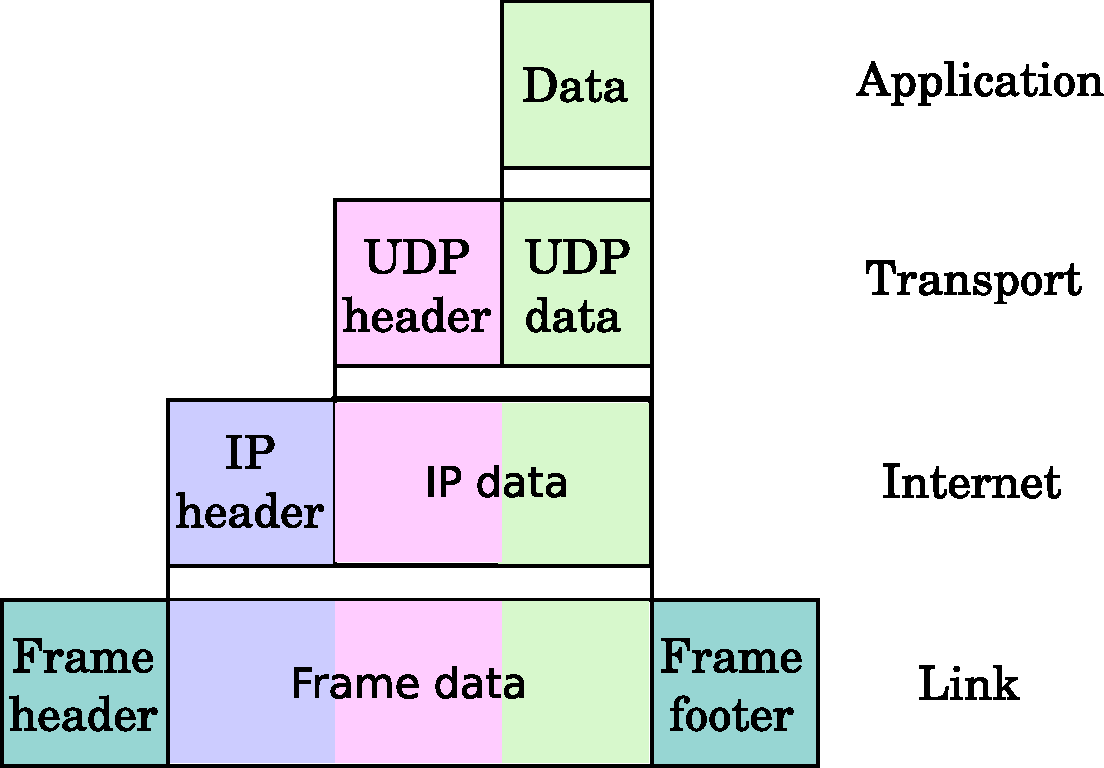
\includegraphics[scale=0.7]{UDP_encapsulation.pdf}
\caption{FIGURA APENAS PARA UDP NAO ESTA CORRECTA ......... Estruturação em camadas baseados em TCP/IP, obtido do sítio da internet http://upload.wikimedia.org/wikipedia/commons/3/3b/UDP\_encapsulation.svg}
\label{fig:stack_tcp_ip}
\end{figure}


A estruturação por camadas permite que a implementação de protocolos seja efectuada de forma simples e rápida, e ao utilizar as camadas inferiores como suporte para as superiores, aumenta a abstracção e complexidade dos protocolos.
Existem vários protocolos de nível transporte sobre \textit{IPv4}, sendo os mais utilizados o \textit{TCP} e \textit{UDP}, como evidencia a figura \ref{fig:stack_tcp_ip}.
A criação de canais sobre o nível de transporte é efectuado utilizando a chamada ao sistema \textit{socket}, indicando para o parâmetro tipo os valores \textit{SOCK\_STREAM} ou \textit{SOCK\_DGRAM} para os protocolos \textit{TCP} e \textit{UDP}, respectivamente.

O \textit{TCP} é utilizado para comunicações com controlo de fluxo de dados, que se adaptam ao canal existente, tolerando a perda momentânea de pacotes, e procedendo à sua retransmissão logo que possível.
O controlo das retransmissões é efectuado através do envio de pacotes (\textit{acknowledges}), que informam o transmissor, dos que foram correctamente recebidos, permitindo-lhe reenviar os que se encontram em falta.

O \textit{UDP} é um protocolo mais leve que o \textit{TCP}, pois não utiliza o controlo anteriormente referido.
Para tal este protocolo é habitualmente utilizado quando se está perante a possibilidade de perda de pacotes durante a transmissão ou quando o controlo da retransmissão destes, é efectuado em camadas superiores.

Para além destes protocolos anteriormente mencionados, existe ainda um protocolo denominado por \textit{SOCK\_RAW}.
Este protocolo permite o acesso directo ao nível rede, através da criação de um canal que comunica directamente com o nível rede da pilha de protocolos \textit{TCP/IP}, permitindo executar protocolos de comunicação em nível utilizador.
Para utilizar \textit{sockets} através do modo \textit{RAW}, é necessário que o utilizador tenha permissões de \textit{super user}, uma vez que neste modo, é permitido ao utilizador específicar parte dos cabeçalhos dos pacotes a enviar, sem que o núcleo os valide.
Contudo, a não validação, pode proporcionar que pacotes maliciosos, isto é, com falhas deliberadas, possam ser introduzidos na rede.
 
\subsubsection{AF\_PACKET}
\label{subsub:af_packet}

A família \textit{AF\_PACKET} comunica directamente com o controlador da interface de rede, possibilitando assim efectuar a monitorização de rede.
A utilização destes \textit{sockets} requer uma autorização de \textit{CAP\_NET\_RAW}, apenas disponível ao \textit{super user}.
Tal verificação previne que utilizadores não autorizados possam monitorizar, ou injectar pacotes na rede, influenciando o seu comportamento.
Dado que dispõe da possibilidade de enviar pacotes directamente para o controlador de rede, uma das suas utilizações é a implementação de protocolos de rede em nível utilizador.
Os de canais da família \textit{AF\_PACKET} são frequentemente utilizado em sistemas de detecção de intrusos, uma vez que permitem analisar os pacotes e detectar falhas na sua formatação.

Como a obtenção dos pacotes por estes canais, é efectuada antes da recepção destes pelos processos, existe a possibilidade de o \textit{NetFilter} bloquear a recepção de alguns pacotes, impedindo as aplicações de os receberem, não obstante este canal já os ter obtido para análise.

Como todos os pacotes recebidos pela(s) interface(s) de rede são obtidos por este canal, é necessário efectuar uma cópia destes e fornece-los à aplicação em nível utilizador.
Esta monitorização implica um peso extra na computação, pelo que diversas técnicas (designadamente \textit{lazy cloning}, \textit{mmap}, etc.) têm sido desenvolvidas no sentido de minimizá-lo.
A utilização de \textit{lazy cloning}, destina-se a apenas efectuar a cópia caso esta seja absolutamente necessária, permitindo reduzir a perda de eficiência do sistema, quando está a monitorizar os pacotes de rede.


%A cópia do pacote é efectuada caso a avaliação do filtro indique que este deve ser copiado, caso contrário é terminada a execução em relação a esse pacote.


\subsection{NetFilter}

Este sistema, está implementado no núcleo do sistema de operação do \textit{Linux}, o qual controla o fluxo de dados dos processos de e para as interfaces de rede.
O \textit{NetFilter} está presente na pilha de protocolos \textit{TCP/IP} em apenas cinco pontos (\textit{PRE ROUTING}, \textit{LOCAL IN}, \textit{FORWARD} \textit{LOCAL OUT} e \textit{POST ROUTING}) onde, em cada um dos quais, existe uma lista de funções a ser executada sobre o pacote, que foi recebido ou transmitido.
Após a finalização destas funções e dependendo do valor retornado, o pacote irá ou não, prosseguir para as restantes camadas, até atingir o \textit{Traffic Control}(apresentado na subseccção \ref{sub:traffic_control}) ou na aplicação, efectuando deste modo o controlo sobre o fluxo de rede.
O \textit{NetFilter} pode ser controlado pelo \textit{iptables}, uma ferramenta em nível utilizador, que através de regras, controla o acesso dos dados das comunicações de rede.

Um dos componentes do \textit{netfilter} designado por \textit{connection tracking}, cuja sua funcionalidade permite que se efectue o acompanhamento das ligações desde a sua iniciação até ao seu término.
De modo a realizar este acompanhamento, este componente necessita de conhecer os diferentes protocolos utilizados.
Do mesmo modo que o \textit{nefilter} pode ser controlado por um programa em nível utilizador, esta componente \textit{connection tracking}, pode igualmente ser controlada pelo administrador, através do \textit{conntrack}.

Este componente, \textit{connection tracking}, permite efectuar uma gestão mais eficiente e inteligente das conexões, sendo geralmente referido como \textit{firewall} com estado, é também utilizada para efectuar \textit{NAT} (\textit{Network Address Translation}) sobre as interfaces de rede.

Na transmissão de dados, quando estes passam no \textit{netfilter}, existe a possibilidade de identificá-los de forma a serem reconhecidos pelo \textit{traffic control}, permitindo assim efectuar uma gestão conjunta e inteligente do tráfego.

\subsection{Traffic Control}
\label{sub:traffic_control}

No núcleo, para além da existência do \textit{NetFilter}, que controla o fluxo de dados na rede, existe o \textit{Traffic Control} que efectua o escalonamento da transferência de dados para o exterior.
Na rede, o escalonamento do tráfego é particularmente importante para os seus administradores, e dado que a largura de banda é um recurso limitado, a sua gestão rigorosa é criteriosamente observada.

A gestão é efectuada através de regras definidas em função da largura de banda, ritmo de envio, ou outros parâmetros.
O tráfego baseado nas regras anteriormente referidas, é agrupado em classes, que podem ter diferentes niveis de prioridade.
Para além desta classificação, é ainda possível definir os algoritmos de escalonamento a utilizar, de modo a potenciar a eficiência da rede.

Quando se verifica a iminencia do envio de um pacote pela função \textit{ip\_output}, este é transmitido para o \textit{Traffic Control}, onde o pacote é marcado com a \textit{tag} da respectiva classe.
Posteriormente, esse pacote irá ser adicionado ao \textit{QDisk} correspondente.
O \textit{QDisk} é a estrutura de suporte à transmissão de dados efectuada pelo \textit{Traffic Control}, onde cada elemento desta estrutura é um \textit{sk\_buff} (que será abordado em \ref{subsub:sk_buff}).


\subsection{Interfaces de rede}

A interface de rede é o dispositivo que efectua a transmissão e recepção de dados na rede.
Do ponto de vista do \textit{cpu}, a interface de rede apenas efectua pedidos de interrupção, sendo que o restante trabalho é realizado pelo controlador de rede, o qual efectua a ponte entre as funcionalidades de rede do núcleo e a interface de rede.

O núcleo mantém a informação sobre as interfaces de rede, inicializadas pelos seus controladores.
Estas, independentemente de estarem ou não em utilização, constam de uma lista duplamente ligada de \textit{net\_devices}.
Em cada posição desta lista existem informações referente a uma interface de rede (nomeadamente a informação sobre o seu endereço \textit{IP}, o seu endereço \textit{MAC}, etc.), bem como outras configurações.

No registo de um novo controlador de interface de rede definem-se as operações a executar em determinados eventos (tais como a recepção e/ou transmissão de frames, a remoção da interface, etc.).
Estas operações são definidas através de uma interface comum (\textit{struct netdev\_ops}), que permite afectar a esta estrutura, funções presentes nos módulos dos controladores, de modo a serem efectuadas as acções necessárias à utilização da interface de rede.

\subsubsection{Estrutura de um sk\_buff}
\label{subsub:sk_buff}

Os dados envolvidos no fluxo de comunicação e utilizados pelos controladores correspondem aos \textit{socket buffers}, estruturas do tipo \textit{sk\_buff}.
Esta estrutura contém diversos elementos, destacando-se os apontadores para a estrutura de rede do controlador, apontadores para secções do pacote (os diversos cabeçalhos pertencentes ao nível de rede e transporte), bem como a dimensão dos espaços alocados para estes e outros apontadores.

\subsection{Captura dos fluxos de dados das interfaces de rede}
\label{sub:network_cap}
O sistema de monitorização de rede, opera de forma opaca à normal utilização da rede, por parte das aplicações.
Desta forma, quando um pacote chega à interface de rede, esta envia ao cpu um pedido de interrupção da computação.
Neste ponto, é desligada a atenção do processador a novas interrupções, passando a computação para o controlador da interface de rede.
Com a atenção do processador a novas interrupções desligada, a computação deve ser breve e restabelecer-se de imediato a atenção do processador, a novas interrupções, para que o normal funcionamento seja retomado.
Apenas a computação crítica é efectuada, diferindo a restante execução através da invocação de um \textit{softirq}, para que seja terminado o tratamento dos pacotes que chegaram à interface.
O escalonamento do \textit{softirq} potencia o aproveitamento dos recursos ao equilibrar a execução de interrupções com as restantes tarefas.

Os pacotes recebidos são entregues aos \textit{sniffers} registados no sistema, antes de o serem aos \textit{packet handlers} respectivos.
A monitorização de rede é efectuada pelos \textit{sniffers}, sendo os pacotes entregues a cada um deles, para que possam proceder à sua análise.
Cada \textit{sniffer} tem um filtro associado escrito em linguagem \textit{bpf}, a ser executado na máquina virtual, implementada para o efeito.

%\subsubsection{Transmissão de dados}

%Uma aplicação em nível utilizador, transfere dados sobre a rede através de chamadas ao sistema de operação, sendo que estas podem ser \textit{send}, \textit{sendto}, \textit{sendmsg}.
%Neste ponto de entrada, os dados são copiados e sobre eles são efectuadas diversas verificações.

%Seguidamente, são utilizadas estruturas e funções do núcleo sobre os dados enviados, fluindo pela \textit{stack TCP/IP} e \textit{netfilter}, até serem entregues ao controlador da interface de rede.

%Os dados gerados pelas diversas camadas da \textit{stack}, são registados numa estrutura \textit{sk\_buffer}, para serem adicionados a um \textit{QDisk}, de modo a serem transmitidos pelo \textit{traffic control}.
%Quando esta ferramenta enviar o pacote para o controlador, é passada a sua referência para os \textit{sniffers} registados, sendo apenas efectuada uma cópia, caso este seja recolhido para análise.
%Os dados passados ao controlador da interface de rede, são transferidos por \textit{DMA} para o dipositivo de rede, e daí para o seu destino.

%Quando a aplicação está a executar e efectua uma chamada ao sistema de operação, este muda de modo e executa no núcleo \color{red} "em nome da aplicação" \color{black}.
%Durante parte da execução da chamada ao sistema de operação, é possível referenciar qual o processo que efectuou a chamada, pois caso esta seja síncrona, é agendado um processamento sobre os dados e a aplicação fica bloqueada aguardando ser re-escalonada através da função \textit{schedule}.
%O sistema de ficheiros mantém a referência sobre quais os canais abertos para cada processo, sendo possível determinar a que processo pertence cada descritor de ficheiro. 

\section{Desenho e arquitectura do MRoP}
\label{sec:mrop_architecture}

O sistema proposto foi desenvolvido procurando cumprir os seguintes requisitos:
\begin{itemize}
\item seleccionar as comunicações que envolvem apenas um processo (ou um conjunto de processos);
\item manter a compatibilidade com o sistema já existente, incrementando a sua funcionalidade;
\item minimizar eventuais perdas de desempenho;
\item a implementação deve envolver poucas alterações ao código do sistema, de modo a facilitar a sua manutenção e evolução a quando das novas versões do sistema \textit{Linux}.
\end{itemize}

Assim, o sistema criado está dividido em quatro componentes principais: filtragem dos pacotes de rede, instrumentação das chamadas ao sistema, repositório do estado das interacções via rede, e controlo e informação sobre o estado da monitorização (ver figura \ref{arquitectura}).
A função de filtragem, invocada por um \textit{hook} que estende o \textit{LSF}, permite que apenas o tráfego do processo alvo seja analisado pelo restante sistema de fitragem do \textit{LSF}.
Por outro lado, relativamente à componente instrumentação das chamadas ao sistema (ou outras funções contidas no sistema de rede), esta actualiza a componente repositório de dados, onde é mantido o estado das interacções via rede do(s) processo(s) alvo, com as efectuadas pelo processo.
Existe ainda um sistema para controlo/configuração, destinado a obter informação sobre o estado da monitorização.

\begin{figure}[htbp]
\begin{center}
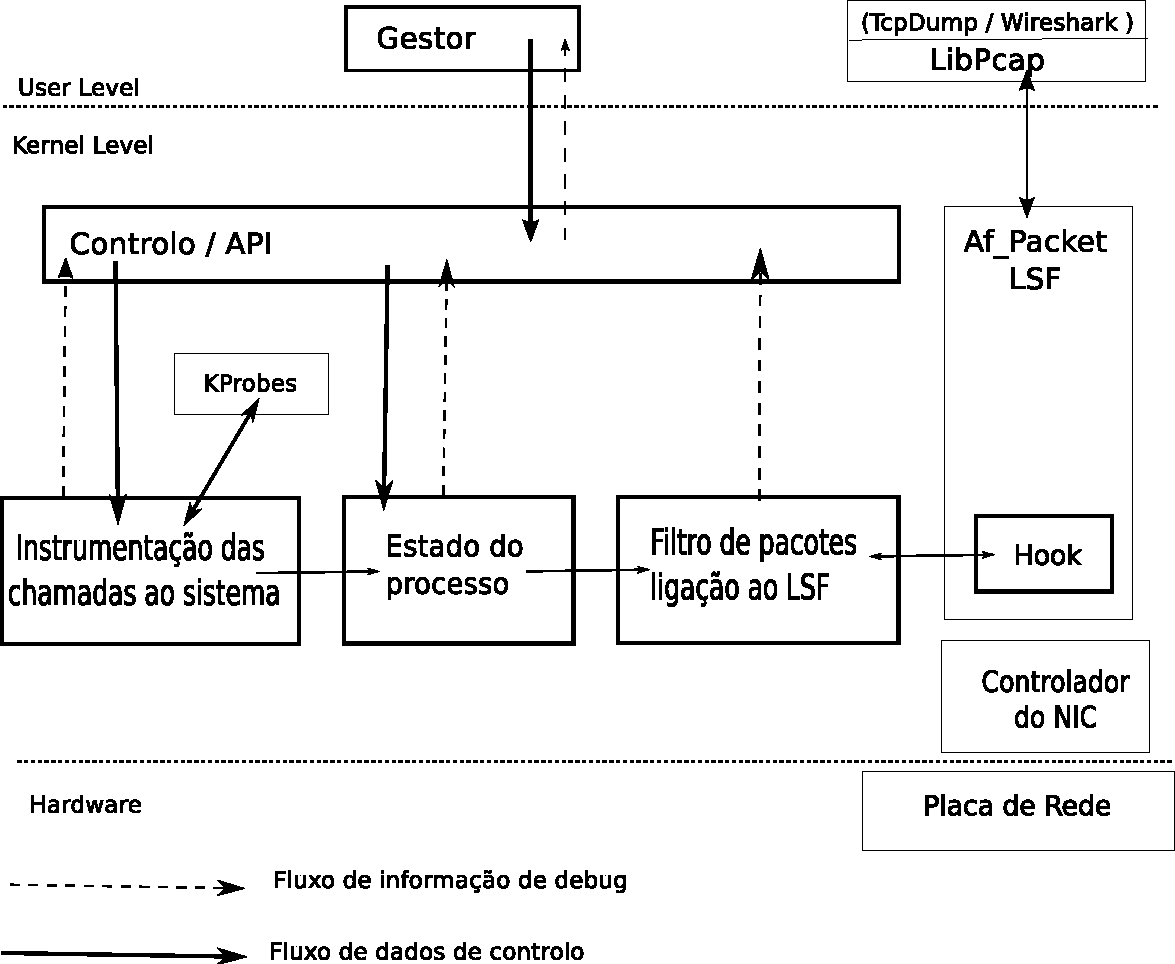
\includegraphics[scale=0.6]{arquitectura.pdf} 
\caption{Arquitectura da solução}
\label{arquitectura}
\end{center}
\end{figure}

Este sistema, \textit{MRoP}, captura os pacotes de rede de um processo, sem que exista um conhecimento prévio sobre o(s) protocolo(s) ou portas utilizadas.
A utilização de um sistema de instrumentação do núcleo foi necessária apenas para monitorizar as chamadas envolvendo \emph{sockets}, e identificar o processo responsável, permitindo desta forma obter e manter permanentemente actualizada a informação relativa ao estado do processo alvo.
De forma a minimizar a redução de desempenho, todo o sistema foi desenvolvido no núcleo do \textit{Linux}, sem alterações nas interfaces já existentes.
Assim, ferramentas que façam uso da biblioteca \textit{LibPCap}, como o programa \textit{tcpdump} ou as suas variantes, podem beneficiar desta extensão sem qualquer alteração e sem impacto relevante no seu desempenho.

Este módulo do núcleo foi desenvolvido em quatro componentes, que em seguida serão apresentados:


\subsection{Instrumentação das chamadas ao sistema de rede}
\label{sub:mon_syscalls}

A principal relevância deste sistema, assenta no pressuposto de que todas as interacções desencadeadas por um processo com o exterior são detectadas.
Para atingir esse objectivo, foi necessário recorrer à monitorização das chamadas ao sistema de rede ao nível do núcleo, possibilitando reduzir as cópias de dados e as trocas de contexto.
Fazendo uso do sistema de monitorização \textit{KProbes}, foi possível realizar a monitorização sob um limitado conjunto de chamadas ao sistema, nomeadamente: \textit{sendto}, \textit{recvfrom}, \textit{bind}, \textit{accept}, \textit{connect} e \textit{close}.
Ao efectuar esta monitorização é possível detectar todas as modificações ao estado dos \textit{sockets} do processo.
Com os dados relevantes obtidos da monitorização, afectados ao repositório, este mantem-se permanentemente actualizado relativamente aos portos, endereços e protocolos, utilizados pela aplicação.
O filtro de pacotes ao aceder ao repositório e ao decidir quais os pacotes a capturar, origina a filtragem dinâmica orientada ao processo.


\subsection{Estado do processo}
\label{sub:data_repository}

O estado dos portos dos protocolos \textit{TCP} e \textit{UDP} em uso no processo alvo, é mantido num repositório de dados e permanentemente actualizado pelo componente anteriormente referido em \ref{sub:mon_syscalls}.
A árvore \textit{Red and Black} já disponível no núcleo do sistema, foi a estrutura dados escolhida para produzir o repositório pretendido.

O conteúdo de cada folha da árvore é uma estrutura com duas listas de elementos, contendo cada uma endereços \textit{IP} utilizados pela aplicação.
A chave de indexação das folhas é o número do porto.
Desta forma, a árvore poderá conter no máximo 65535 elementos, por ser este o número máximo de portos em utilização por um endereço \textit{IP}.
No pior caso, a procura de um porto na árvore necessitará de efectuar dezasseis iterações, uma vez que \begin{math}\log _2 65536 = 16 \end{math}.

O uso deste tipo de estrutura, permite obter um bom compromisso entre o tempo de acesso aos dados e a quantidade de memória utilizada.

\subsection{Filtro de pacotes}
\label{sub:packet_filter}

A função de filtragem implementada neste sistema assenta no estado do processo alvo, mantido pelos módulos anteriormente descritos.
Através da extensão do \textit{LSF} com um \textit{hook}, este quando ligado, invoca esta filtragem que devolve uma resposta ao \textit{LSF}, informando-o se deve ou não capturar o pacote em causa.
Caso seja capturado indica que este pertence ao processo alvo, caso contrário irá ser sujeito a um processo de avaliação, baseado nas restantes regras de filtragem definidas.
Mantêm-se assim, a compatibilidade e os benefícios da utilização do \textit{Linux Socket Filter}.
Quando não existe uma ligação (\textit{hook}) activa, assiste-se a um ligeiro decréscimo no desempenho na utilização da filtragem estática.
Tal facto deve-se apenas à necessidade de constatar se a ligação (\textit{hook}) está ou não activa.

Como se verifica, este sistema interage com o filtro estático do \textit{LSF}, efectuando uma conjunção entre o filtro definido pelo utilizador e a captura do tráfego da aplicação a ser monitorizada.

\subsection{Controlo e Informação}
\label{sub:data_information}

Para facilmente controlar e configurar o sistema desenvolvido, foi definida uma interface baseada em ficheiros virtuais, numa directoria do (\textit{DebugFS}).
Esta interface que contém ficheiros para indicar ao \textit{MRoP} quais os identificadores do processo a monitorizar, permite ao administrador obter informações estatísticas da monitorização, bem como controlar o repositório de dados do estado do processo.
É através desta interface, que os actuais sistemas de monitorização de rede, podem usufruir da funcionalidade disponível através do \textit{MRoP}.

Estes ficheiros com permissões apenas acessíveis ao utilizador \textit{root}, impedem o acesso por parte dos restantes utilizadores da máquina ao sistema de monitorização.

\section{Conclusão}

Algumas ideias para concluir este capitulo ...

